\chapter{Programmbeschreibung} % (fold)
\label{chap:Programmbeschreibung}

Im Folgenden soll eine Programmbeschreibung für die Portfolioaufgabe von Verteilte Systeme aus dem 4. Semester erstellt werden.

Das Programmsystem wurde auf einem Linux Debian 12 Computer geschrieben und getestet.
Es wurde ein Firefox Browser und der Tomcat Server mit der Version Apache Tomcat/9.0.70 (Debian) verwendet.

JSPs wurden grundsätzlich für den Bestellvorgang verwendet, da hier sehr gut mit HTML-Funktionen gearbeitet werden kann und die Einbindung von Beans recht leicht und flüssig funktioniert.
Bei der Rechnungserstellung wird auf Grund der vielen Logik und der mathematischen Rechnungen auf Servlets gesetzt.
Sie erlauben übersichtlicheren und unkomplizierteren Programmcode, da direkt mit Java gearbeitet wird und keine Tags verwendet werden müssen.

\section{Index.jsp} % (fold)
\label{sec:Index.jsp}

Die Index.jsp Seite ist die Einstiegsseite des Programmsystems, dass ich Bestellung 3000 genannt habe.
Sie beinhaltet eine kurze Erklärung zum Sinn des Programmsystems und zur rudimentären Funktionsweise (siehe Abbildung~\ref{abb:IndexJSP}).

\begin{figure}[htb]
  \centering
  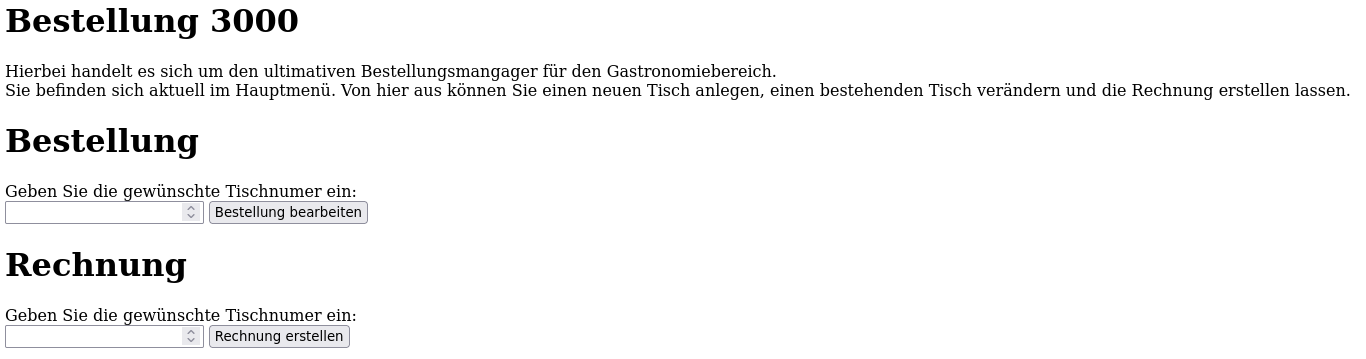
\includegraphics[width=0.95\textwidth]{images/IndexJSP.png}
  \caption[Index.jsp]{Index.jsp}
  \label{abb:IndexJSP}
\end{figure}

Um eine Bestellung aufzugeben, oder eine bestehende Bestellung zu bearbeiten muss unter \textit{Bestellung} eine gültige Tischnummer eingegeben werden und mit dem Knopf \textit{Bestellung bearbeiten} bestätigt werden.
Gültige Tischnummern sind 1 bis 5, da mein Programmsystem mit 5 verschiedenen Tischen arbeitet.
Zum genauen Ablauf von der Aufgabe und der Veränderung einer Bestellung mehr unter Abschnitt~\ref{sec:Bestellungen aufgeben} und \ref{sec:Bestellungen verändern}.

Rechnungen können Benutzer unter \textit{Rechnung} erstellen lassen.
Auch hier muss eine gültige Tischnummer eingegeben werden, die mit dem Knopf \textit{Rechnung erstellen} bestätigt wird.
Wie genau Rechnungen funktionieren, und welche Funktionen Teil der Rechnungserstellung sind steht in Abschnitt~\ref{sec:Rechnungen}

% section Index.jsp (end)

\section{Datenspeicherung} % (fold)
\label{sec:Datenspeicherung}

Die temporäre Datenspeicherung findet aus einem Zusammenspiel von einer Bean-Klasse namens FormBean.java und Sessionvariablen statt.
Da ein Objekt der FormBean-Klasse in der Session gespeichert wird, sind quasi alle Daten in der Session gespeichert.

Im FormBean-Objekt werden alle Daten zu den Tischen gespeichert.
Codeblock~\ref{lst:Bestellungsspeicherung} zeigt, wie die Daten in Form eines zweidimensionalen Arrays gespeichert wird.

\begin{lstlisting}[language=java, caption=Bestellungsspeicherung, label=lst:Bestellungsspeicherung]
  int[][] tische = new int[5][10];
\end{lstlisting}

Die erste Dimension steht für die Anzahl der Tische.
Im Array tische mit dem Index 0 (tische[0]) werden die Anzahlen für die Produkte, die Tisch 1 bestellt hat, gespeichert.
Dies ist beim Setzen der Produktanzahlen zu beachten, die Auswirkungen daraus werden in Codeblock~\ref{lst:GetterUndSetter} deutlich.

Für jedes der Produkte muss eine Getter- und eine Setter-Methode definiert werden.
Codeblock~\ref{lst:GetterUndSetter} zeigt diese Idee beispielhaft.
Die Anzahl der bestellten Colas wird in der zweiten Dimension des Arrays tische mit dem Index 0 gespeichert, also wie in der setAnzahlCola-Methode.

\begin{lstlisting}[language=java, caption=Beispiel für Getter- und Setter-Methoden, label=lst:GetterUndSetter]
  public int getAnzahlCola() {
    return tische[tischNr - 1][0];
  }

  public void setAnzahlCola(int anzahlCola) {
    tische[tischNr - 1][0] = anzahlCola;
  }
\end{lstlisting}

Daten, die nicht direkt Teil einer Bestellung sind, wie der Rabatt, oder welche Person welche Produkte bezahlt werden an gegebener Stelle separat in der Session gespeichert.

% section Datenspeicherung (end)

\section{Bestellungen aufgeben} % (fold)
\label{sec:Bestellungen aufgeben}

\begin{figure}[htb]
  \centering
  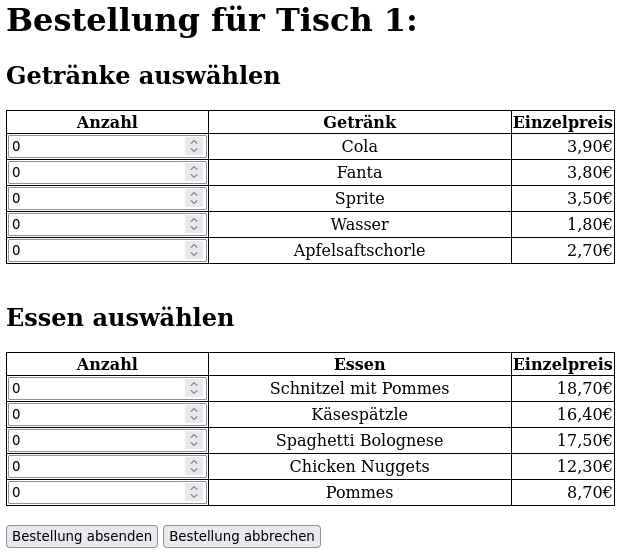
\includegraphics[height=8cm]{images/InitialBestellungJSP.png}
  \caption[Bestellung.jsp bei erster Bestellung]{Bestellung.jsp bei erster Bestellung}
  \label{abb:InitialBestellungJSP}
\end{figure}

Wenn, wie bereits beschrieben, der Benutzer eine Bestellung aufgeben will, öffnet sich die Bestellung.jsp.
Die Maske dieser Seite ist in Abbildung~\ref{abb:InitialBestellungJSP} sichtbar.

Die bestellbaren Produkte sind hier in zwei Tabellen aufgeteilt, eine für Getränke und eine für Essen.
Die erste Spalte beider Tabellen erlaubt eine Eingabe der gewünschten zu bestellenden Anzahl.
Die zweite Spalte listet jeweils die Getränke oder Essen auf und in der dritten Zeile sind die Einzelpreise der Produkte aufgelistet.

Bestellt ein Tisch also beispielsweise vier Colas, ein Schnitzel mit Pommes und drei mal Käsespätzle, muss der Benutzer nur die richtige Zahl an der jeweiligen Stelle eingeben.
Bestätigt wird die Bestellung mit dem Button \textit{Bestellung absenden}.
Erst dann werden die eingegebenen Daten gespeichert und der Benutzer wird auf die Startseite zurückgeleitet.
Der Button \textit{Bestellung abbrechen} leitet den Benutzer ebenfalls zurück zur Startseite, die Daten werden dann natürlich nicht verworfen.

% section Bestellungen aufgeben (end)

\section{Bestellungen verändern} % (fold)
\label{sec:Bestellungen verändern}

Beim Verändern von Bestellungen wird die selbe Seite aufgerufen.
Wenn auf dem ausgewählten Tisch (in der Überschrift ist die ausgewählte Tischnummer sichtbar) bereits Produkte bestellt wurden, sind die absoluten Werte der bestellten Produkte der Wert der Anzahl Eingabefelder.

\begin{figure}[htb]
  \centering
  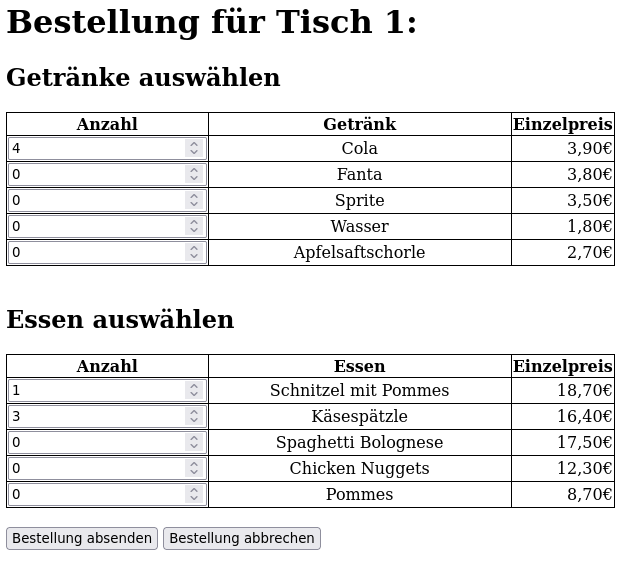
\includegraphics[height=8cm]{images/ChangeBestellungJSP.png}
  \caption[Bestellung.jsp bei Bestellungsveränderung]{Bestellung.jsp bei Bestellungsveränderung}
  \label{abb:ChangeBestellungJSP}
\end{figure}

Um das Beispiel von oben aufzunehmen, sind in Abbildung~\ref{abb:ChangeBestellungJSP} die zuvor bestellten vier Colas, drei Käsespätzle und das eine Schnitzel mit Pommes sichtbar.
Nun können jegliche Veränderungen vorgenommen werden.
Angenommen, anstatt der vier Colas wurden nur drei bestellt und eine Fanta, aber der Benutzer hatte sie zuvor falsch eingetragen.
Außerdem wurde noch eine Portion Chicken Nuggets nachbestellt.
Der Benutzer muss nun einfach die aktuellen absoluten Werte eingeben und die Bestellung absenden.

% section Bestellungen verändern (end)

\section{Rechnungen} % (fold)
\label{sec:Rechnungen}

\subsection{Auswahl der Rechnungserstellung} % (fold)
\label{sub:Auswahl der Rechnungserstellung}

Wenn eine Rechnung für beispielsweise Tisch 2 erstellt werden soll, für diesen Tisch aber noch keine Produkte bestellt wurden wird die Fehlermeldung von Abbildung~\ref{abb:RechnungFehler} ausgegeben.

\begin{figure}[htb]
  \centering
  
\includegraphics[width=0.95\textwidth]{images/RechnungFehler.png}
  \caption[Fehlermeldung bei Rechnungserstellung]{Fehlermeldung bei Rechnungserstellung}
  \label{abb:RechnungFehler}
\end{figure}

Mit dem Button \textit{Zurück zur Startseite} wird die Fehlermeldung bestätigt, und der Benutzer wird zur Startseite zurückgeleitet.

Wenn eine valide Rechnung erstellt werden kann, wird der Benutzer aufgefordert anzugeben, ob die Kunden zusammen oder getrennt zahlen wollen.
Dieses Feld ist ein Pflichtfeld, um eine weitere Erstellung der Rechnung zu erlauben.

\begin{figure}[htb]
  \centering
  
\includegraphics[width=0.95\textwidth]{images/InitialRechnung.png}
  \caption[Erste Seite der Rechnungserstellung]{Erste Seite der Rechnungserstellung}
  \label{abb:InitialRechnung}
\end{figure}

Wie in Abbildung~\ref{abb:InitialRechnung} sichtbar gibt es noch ein zweites Feld.
In dieses kann ein Rabattcode eingegeben werden.
Nur die drei Rabattcodes "Rabatt1", "Rabatt2"\ und "Rabatt3"\ sind valide.
Codeblock~\ref{lst:RabattFeld} zeigt, wie das mit Hilfe des Setzen eines patterns garantiert wird.

\begin{lstlisting}[language=html, caption=Eingabefeld für den Rabattcode, label=lst:RabattFeld]
  <input type="text" name="rabatt" pattern="Rabatt1|Rabatt2|Rabatt3">
\end{lstlisting}

Beim \textit{Bestätigen} dieser Angaben wird der Rabatt als Sessionvariable gespeichert und der Benutzer wird entweder auf das RechnungZusammen-Servlet, oder auf das RechnungGetrennt-Servlet umgeleitet.

% subsection Auswahl der Rechnungserstellung (end)

\subsection{Rechnungen zusammen begleichen} % (fold)
\label{sub:Rechnungen zusammen begleichen}

Wollen die Kunden zusammen bezahlen sieht der Benutzer Abbildung~\ref{abb:RechnungZusammen}.
Hier wird ein detailierter Überblick über die Rechnung gegeben.
In der linken Spalte wird der Name des Produkts aufgelistet, in der mittleren wird die jeweilige Menge und in der rechten der Preis für die jeweilige Zeile aufgelistet.
In grüner Schrift hervorgehoben ist der durch den Rabatt, in diesem Fall 30\% durch den Rabattcode "Rabatt3", gutgeschriebene Geldbetrag angegeben.
In der letzten Zeile der Rechnung wird der zu zahlende Betrag, in roter Schrift hervorgehoben, angezeigt.

\begin{figure}[htb]
  \centering
  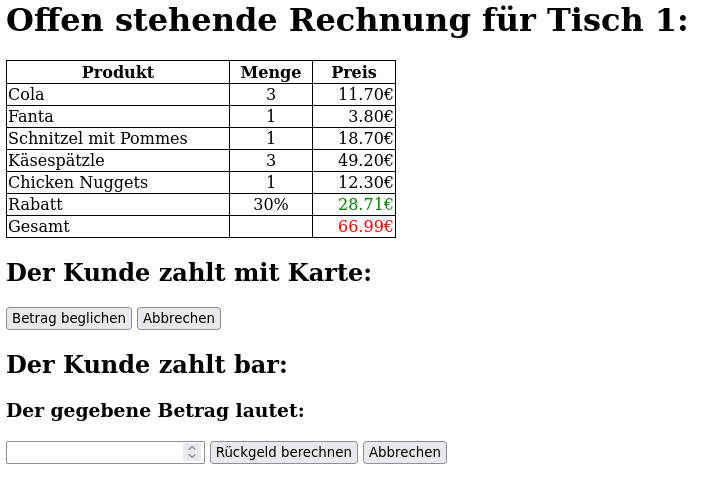
\includegraphics[height=8cm]{images/RechnungZusammenServlet.png}
  \caption[Rechnung-Zusammen-Servlet]{Rechnung-Zusammen-Servlet}
  \label{abb:RechnungZusammen}
\end{figure}

Der Kunde hat nun die Möglichkeit mit Karte oder bar zu bezahlen.
Wählt der Kunde Kartenzahlung, so werden mit dem Button \textit{Betrag beglichen} alle bestellten Produkte von, in diesem Fall, Tisch 1 gelöscht und der Benutzer wird auf die Startseite zurückgeleitet.
Entscheidet sich der Kunde für Barzahlung, muss ein Geldbetrag eingetragen werden, den der Kunde gegeben hat.
Das Eingabefeld lässt nur Werte zu, die größer als der zu zahlende Betrag sind, um zu garantieren, dass die Rechnung beglichen werden kann.
Mit \textit{Rückgeld berechnen} wird dem Benutzer Abbildung~\ref{abb:BarZusammen} angezeigt.

\begin{figure}[htb]
  \centering
  
\includegraphics[width=0.95\textwidth]{images/RechnungZusammenBarServlet.png}
  \caption[Rückgeldberechnung]{Rückgeldberechnung}
  \label{abb:BarZusammen}
\end{figure}

Erst, wenn der Button \textit{Rückgeld gegeben} gedrückt wird, wird die Bestellung gelöscht und der Benutzer auf die Startseite zurückgeleitet.
Zu jedem Zeitpunkt dieses Vorgangs kann dieser abgebrochen werden und der Benutzer wird an den jeweils vorherigen Schritt zurückgeführt.

% subsection Rechnungen zusammen begleichen (end)

\subsection{Rechnung getrennt begleichen} % (fold)
\label{sub:Rechnung getrennt begleichen}

Wenn getrennte Rechnungen gewünscht sind, wird Abbildung~\ref{abb:RechnungGetrennt} angezeigt.
Die Darstellung der Rechnung ist ähnlich, wie bei zusammen gezahlten Rechnungen.
Die ersten drei Spalten sind die selben, in der vierten Zeile wird allerdings zusätzlich eine Spalte mit Eingabefeldern ausgegeben.
In diesen kann angegeben werden, was eine Person zahlt.

\begin{figure}[htb]
  \centering
  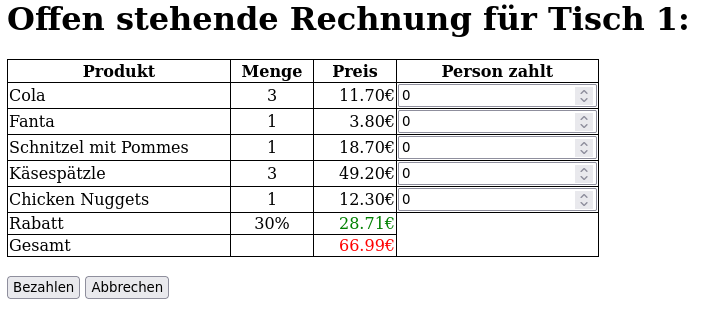
\includegraphics[width=0.75\textwidth]{images/RechnungGetrenntServlet.png}
  \caption[Rechung-Getrennt-Servlet]{Rechung-Getrennt-Servlet}
  \label{abb:RechnungGetrennt}
\end{figure}

Beispielsweise zahlt Person 1 eine Cola und das Schnitzel mit Pommes.
Mit dem Button \textit{Bezahlen} wird diese Angabe bestätigt.
Resultierend daraus entsteht Abbildung~\ref{abb:RechnungGetrenntZahlen}.

\begin{figure}[htb]
  \centering
  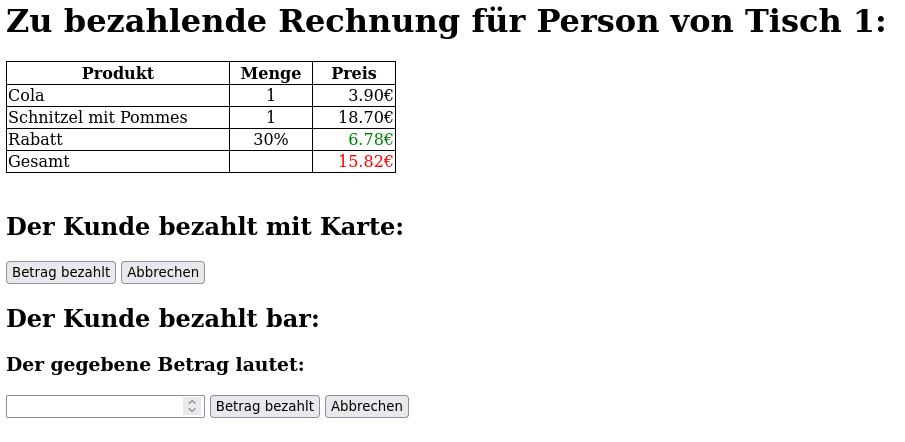
\includegraphics[width=0.95\textwidth]{images/RechnungGetrenntZahlen.png}
  \caption[Rechnung für eine Person]{Rechnung für eine Person}
  \label{abb:RechnungGetrenntZahlen}
\end{figure}

Auf dieser Seite wird nochmal eine Rechnung für diese eine Person erstellt.
Das Bezahlen funktioniert parallel zum Zusammenzahlen und erlaubt auch Kartenzahlung und Barzahlung.
Wenn nach bezahlen der Teilrechnung noch offene Produkte auf dem Tisch gebucht sind wird der Benutzer zurück zur Gesamtrechnung (Abbildung~\ref{abb:RechnungGetrennt}) geleitet und kann die nächste Person abrechnen.
Ansonsten wird der Benutzer direkt auf die Startseite geleitet.

% subsection Rechnung getrennt begleichen (end)

% section Rechnungen (end)

\section{Die Util-Klasse} % (fold)
\label{sec:Die Util-Klasse}

Die Util-Klasse fungiert als eine Sammlung von Methoden, die an mehreren Stellen des Programmsystems Anwendung finden und deshalb an einem Ort gesammelt und bereitgestellt werden.
Für genauere Informationen zu den einzelnen Methoden und deren Funktionsweise, ist der Code ausführlich kommentiert.

% section Die Util-Klasse (end)

% chapter Seitenübersicht (end)

